\RequirePackage{amsthm}

\documentclass[sn-vancouver,Numbered]{sn-jnl}



\usepackage{graphicx}%
\usepackage{multirow}%
\usepackage{amsmath,amssymb,amsfonts}%
\usepackage{amsthm}%
\usepackage{mathrsfs}%
\usepackage[title]{appendix}%
\usepackage{xcolor}%
\usepackage{textcomp}%
\usepackage{manyfoot}%
\usepackage{booktabs}%
\usepackage{algorithm}%
\usepackage{algorithmicx}%
\usepackage{algpseudocode}%
\usepackage{listings}%

\usepackage{tikz}
\usetikzlibrary{arrows.meta, positioning, fit, backgrounds, calc}


%% as per the requirement new theorem styles can be included as shown below
\theoremstyle{thmstyleone}%
\newtheorem{theorem}{Theorem}%  meant for continuous numbers
%%\newtheorem{theorem}{Theorem}[section]% meant for sectionwise numbers
%% optional argument [theorem] produces theorem numbering sequence instead of independent numbers for Proposition
\newtheorem{proposition}[theorem]{Proposition}% 
%%\newtheorem{proposition}{Proposition}% to get separate numbers for theorem and proposition etc.

\theoremstyle{thmstyletwo}%
\newtheorem{example}{Example}%
\newtheorem{remark}{Remark}%

\theoremstyle{thmstylethree}%
\newtheorem{definition}{Definition}%

\raggedbottom
\bibpunct{[}{]}{,}{n}{,}{,}
%%\unnumbered% uncomment this for unnumbered level heads

\begin{document}

\title[Article Title]{A Novel Computational Framework for $\S2$ Voting Rights Act Analysis}


\author*[1]{\fnm{Alicia} \sur{Guerra}}\email{aguerra4@hawk.illinoistech.edu}

\affil*[1]{\orgdiv{College of Computing}, \orgname{Illinois Institue of Technology}, \orgaddress{\street{10 W 35th Street}, \city{Chicago}, \postcode{60616}, \state{Illinois}, \country{United States}}}



\abstract{A modular computational framework for $\S2$ Voting Rights Act is introduced which integrates geospatial data engineering, Bayesian ecological inference, and ensemble generation. Prior work has developed these components individually, existing approaches lack a unified pipeline that propagates uncertainty from voter behavior estimation through plan-level evaluation. A probabilistic notion of minoirty electoral opportunity is formalized. A case study of Texas congressional districts illustrates how the framework can be used to assess whether an enacted plan systematically dilutes minoirty voting power.}

\keywords{racial gerrymandering, computational redistricting, ecological inference, redistricting ensembles, Bayesian hierarchical modeling, racially polarized voting, Voting Rights Act, minority vote dilution}

\maketitle

\section{Introduction}\label{sec1}

\subsection{Redistricting in the United States}
After the decennial U.S. census and apportionment is conducted, states usually initiate their redistricting processes, during which they formulate district boundaries accounting for population changes that occured during the past decade \cite{EckmanWhitaker2025MidDecade}.

Although redistricting processes are mostly determined by state laws, congressional district maps are required to comply with the the U.S. Constitution and federal law \cite{EckmanWhitaker2025MidDecade}.

Since the 1964 Wesberry v. Sanders decision, the U.S. Supreme Court has interpreted the Constitution as mandating that every congressional district possess approximately the same number of people \cite{EckmanWhitaker2025MidDecade}. The population totals are obtained from the U.S. Census; nowadays,all congressional districts in a state have a population difference of zero or at most one \cite{Duchin2023PoliticalGeometry}.

Furthermore, the majority of states require that congressional districts be compact and contiguous - that is, that their districts be reasonably shaped and have all their portions be geographically connected, respectively \cite{Duchin2023PoliticalGeometry}. Although not all states explicitly require compactness and contiguity in their Constitutions, this is considered "standard practice" \cite{deford2021recombination}. The U.S. Supreme Court treats compactness and contiguity as traditional redistricting principles and diagnostic signals in racial gerrymandering analysis. For instance, in cases such as Shaw v. Reno \cite{Shaw1993}, Miller v. Johnson \cite{Miller1995}, and Bush v. Vera \cite{Bush1996}, lack of compactness and contiguity were cited as evidence of race predominantly determining district lines, which is required to prove racial gerrymandering in violation of the 14th Ammendment.

\subsubsection{Gerrymandering}
Gerrymandering is a tactic that has been interwoven with United States politics since at least 1812, which is when the term was first coined. In simplest terms, gerrymandering can be defined as the manipulation of election district maps to either favor or disfavor a group of people (i.e. a political party, a racial/ethnic group, a socioeconomic class, etc). 

\subsubsection{Negative Racial Gerrymandering}
Negative racial gerrymandering dilutes minority voting power by engineering districts in which minority ballots systematically matter less. Although minority voters retain the formal right to vote, they lack proportional influence.

This distortion produces legislatures that are less representative—often whiter and more ideologically extreme than the electorate—and weakens elected officials’ incentives to respond to minority interests.

By breaking the link between voting and representation, negative racial gerrymandering undermines democratic legitimacy, erodes trust, and contributes to lower turnout and political disengagement.

\subsubsection{The Legality of Negative Racial Gerrymandering}
\label{sec:legality}
Negative racial gerrymandering is illegal in the United States by virtue of the Equal Protection Clause of the Fourteenth Ammendment and $\S2$ of the Voting Rights Act. 

The Equal Protection Clause of the Fourteenth Ammendment forbids denying anyone of "equal protections of the law" \cite{USConst14}.

Section 2 of the Voting Rights Act of 1965 precludes states and political entities from wielding any "standard, practice, or procedure" to curtail the voting rights of any U.S. citizen based on race \cite{vra1965_sec2}. In the 1986 case of Thornburg v. Gingles, it was ruled that a North Carolina redistricting plan was in violation of $\S$2 of the Voting Rights Act for engaging in negative racial gerrymandering practices - more specifically, of diluting the votes of black citizens \cite{thornburg1986gingles}. This landmark Supreme Court case decided that minority voters can legally challenge negative racial gerrymandering practices in redistricting plans on the grounds of violating $\S$2 of the Voting Rights Act, but that the burden of proof is on them to demonstrate that their capacity to elect their preferred candidates is undermined \cite{thornburg1986gingles}. 

In the Thornburg v. Gingles case, the Supreme Court established a framework for minority voters to be able to prove negative racial gerrymandering in violation of $\S$2 of the Voting Rights Act in a court of law \cite{thornburg1986gingles}. Under this framework, plantiffs must be able to prove the following: (1) a "geographically insular" minority group makes up the majority population of a district, (2) the minority group is "politically cohesive", and (3) the "bloc voting majority" is usually able to defeat the minority group's preferred candidates \cite{thornburg1986gingles}. The second and third preconditions are stated by the U.S. Supreme Court as concerning "racially polarized voting" \cite{allen_milligan_2023}.

The U.S. Supreme Court refers to this framework as "the Gingles framework" \cite{allen_milligan_2023}. For the last 40 years, claims of negative racial gerrymandering in violation of $\S$ of the Voting Rights Act have been assessed via the Gingles framework \cite{allen_milligan_2023}. In the 2023 Allen v. Milligan decision, the U.S. Supreme Court reaffirmed the validity of the Gingles framework \cite{allen_milligan_2023}.

\section{Related Work and Contribution}\label{sec2}
\subsection{Redistricting Data Preparation}
\subsubsection{Constructing Demographic Categories}
In this paper, the Data and Democracy Lab's conventions for constructing demographic categories are adopted. 

Their convention for categorizing racial groups inolves adopting these group names in the ensuing order: Black, Hispanic, Asian, Other,and White \cite{mggg_vap_cvap}. 

It is emphasized that anyone who identifies as black should be grouped into the black population \cite{mggg_vap_cvap}. In other words, the black population should encompass those who are "Any-Part Black" or "Black Alone or in Combination", as opposed to just "Black Alone" or "Single-Race Black" \cite{mggg_vap_cvap}. 

Then, of the individuals left, the Hispanic population must encompass all individuals who identify as Hispanic in the same way the Black population does \cite{mggg_vap_cvap}. Next, of those left, the Asian population should capture all who identify as Asian or Native Hawaiin Pacific Islander, so as to represent an AAPI category \cite{mggg_vap_cvap}. Finally, the same logic is used to construct the AMIN, Other, and White categories \cite{mggg_vap_cvap}.

Thereafter, source \ref{data:pl94} in Section~\ref{sec:datasources} is leveraged to generate voting age population as sums of census variables \cite{mggg_vap_cvap}.

Subsequently, Source \ref{data:cvap} in Section~\ref{sec:datasources} is analyzed. The problem is, CVAP data from the ACS must be analyzed at the census block level because the base unit of the Decennial Census PL 94-171 data is the census block. In the primary tables, ACS is reported at the census tract level, which presents a problem because that is a significantly higher level of aggregation than the census block \cite{mggg_vap_cvap}.

Fortunately, the Data and Democracy Lab has introduced a solution to this problem called "discounting" \cite{mggg_vap_cvap}. Discounting refers to the usage of the tract-level ACS data to estimate the citizenship rates of racial groups, then applying the discount to the voting age population \cite{mggg_vap_cvap}.

An example of "discounting" provided by the Data and Democracy Lab is depicted in Equation~\ref{eq:discounting}; in this example, block X belongs to tract Y in state Z and BCVAP is estimated by taking the citizenship rate for the group in the tract and applying it to the voting ager population in the block \cite{mggg_vap_cvap}.
\begin{equation}
\frac{BCVAP_{ACS}(tract \: Y)}{BVAP_{ACS}(tract \: Y)} \times BVAP_{PL}(block \: X) = BCVAP(block \: X)
\label{eq:discounting}
\end{equation}

If the denominator in an equation like Equation~\ref{eq:discounting} is too low, then the Data and Democracy Lab proposes a solution like that in Equation~\ref{eq:discounting_fix}. This involves swapping in the citizenship rate given that the tract did not allow for a meaninful estimate \cite{mggg_vap_cvap}.

\begin{equation}
\frac{BCVAP_{ACS}(state \: Z)}{BVAP_{ACS}(state \: Z)} \times BVAP_{PL}(block \: X) = BCVAP(block \: X)
\label{eq:discounting_fix}
\end{equation}

The Data and Democracy Lab acknowledges that this is a "crude fix", but states that they intend to release a "more sophisticated" Bayesian method to address this in the future \cite{mggg_vap_cvap}. 

\subsection{Ecological Inference}
To reiterate what is stated in $\S$~\ref{sec:legality}, in order to prove a violation of $\S2$ of the Voting Rights Act under the Gingles framework,plaintiffs must prove that the majority votes as a bloc to defeat minority-preferred candidates \cite{thornburg1986gingles}. Hence, any framework performing $\S2$ Voting Rights Act analysis must encompass identification of minority-preferred political candidates \cite{BeckerDuchinGoldHirsch2021}.

In state election return datasets, vote totals for political candidates are not computed by race, meaning that direct computation of minority-preferred candidates is impossible \cite{BeckerDuchinGoldHirsch2021}. This is where ecological inference - the de-facto solution for determining racially polarized voting - comes in. After all, ecological inference is widely regarded as "the best and often only hope of making progress" when it comes to extracting clues about individual behavior from group or aggregate-level data \cite{king2004ecological}.

Ecological inference (and ecological regression, its simpler predecessor) is considered a "statistical mainstay" in $\S2$ Voting Rights Act litigation \cite{freedman1999ecological}. U.S. Supreme Court redistricting cases in which lower-court findings relying on ecological inference were reviewed and accepted without methodological objection include Allen v. Milligan \cite{allen_milligan_2023}, Alexander v. State Carolina State Conference of the NAACP \cite{alexander2024}, Cooper v. Harris \cite{cooper2017}, Bethune-Hill v. Virginia State Board of Elections \cite{bethunehill2017}, and Abbott v. Perez \cite{abbott2018}.

It should be noted, however, that in the same way all statistical inference techniques with missing data give way to uncertainty, ecological inference produces "imperfect" and "uncertain" answers \cite{BeckerDuchinGoldHirsch2021}. Hence, it is essential to estimate the error produced by ecological inference techniques and observe how it compounds or cancels out in high-level conclusions \cite{BeckerDuchinGoldHirsch2021}.So, in addition to identifying the minority-preferred candidates, one must specify the confidence measures that the identifications are correct \cite{BeckerDuchinGoldHirsch2021}. To check for minoirty control of a district and identify preferred candidates for newly proposed districts, the statewide and precinct-level vote estimates by race should be leveraged \cite{BeckerDuchinGoldHirsch2021}.

Becker et al. \cite{BeckerDuchinGoldHirsch2021} implement a version of King's ecological inference, specifically the ei.mD.bayes function from eiPack which is based on the Bayesian hierarchical Dirichlet model for $R \times C$ tables proposed by King et al. in 1999 \cite{king1999binomial_beta_ei}. 

For each election, EI is run at the statewide level using precinct-level input tables \cite{BeckerDuchinGoldHirsch2021}. The inputs for each precinct are the row and column sums for the $R \times C$ table of vote counts. The row sums correspond to the precinct's estimated number of adult citizens in each racial group. The column sums are the precinct's vote totals for each candidate \cite{BeckerDuchinGoldHirsch2021}.

Each ecological inference run generates a large random sample of estimated vote counts; in order to obtain the statewide estimates, these values are summed across the entire state \cite{BeckerDuchinGoldHirsch2021}. For each racial group, the candidate with the highest average estimanted vote total for an election is the preferred candidate \cite{BeckerDuchinGoldHirsch2021}. In order to obtain a measure of confidence for the a candidate was correctly identified as the preferred candidate, repeated draws for the ecological inference ditribution are obtained and the frequency by which the preferred candidate recieves the most votes is recorded \cite{BeckerDuchinGoldHirsch2021}.

\subsection{Ensemble Methods}
Recent methods for analyzing and comparing districting plans attempt to do so by placing a plan in the context of valid alternatives - that is, those that cut up the same jurisdiction by the same rules and with the sturctural features of the geography and the pattern of voting held constant \cite{deford2021recombination}. These ensembles contain samples from the full space of plans, aiming to help compare a plan's properties to the range of possible designs \cite{deford2021recombination}. 

In one powerful application, ensembles have been used to conduct outlier analysis, or to argue that a proposed plan has properties that are extreme relative to the comparison statistics of alternative plans \cite{deford2021recombination}. Arguments like this have featured in a string of recent legal challenges to partisan gerrymanders, all of which were successful at the district court or Supreme Court level \cite{deford2021recombination}. Outliers have also recieved significant attention from the U.S. Supreme Court (culminating in Rucho v. Common Cause), but a 5-4 majority declared that it was too hard for a federal court to decide how much is too much of an outlier \cite{deford2021recombination}. Outside of federal courts, the method is very much alive not only in state-level legal challenges but as a screening step for the initial adoption of plans, and we expect numerous states to employ ensemble analysis this year when new plans are enacted around the country \cite{deford2021recombination}.

In the past 5 years, researchers have turned to Markov chain Monte Carlo for sampling \cite{deford2021recombination}. MCMC methods offer strong underlying theory and heuristics, in the form of mixing theorems and convergence diagnostics \cite{deford2021recombination}. The idea is to form a random walk on the state space and collect states visited by the walker to build a sample \cite{deford2021recombination}. The first and most natural approach to defining a random walk on graph partitions is to simply reassign one node at a time through a random process called a flip process \cite{deford2021recombintion}. 

\subsubsection{Recombination Markov Chains}
In 2021, Daryl DeFord, Moon Duchin, and Justin Solomon set forth recombination, a novel family of Markov chains intended for the ensemble generation of alternative redistricting plans \cite{deford2021recombination}. Recombination has become the standard engine for district plan ensemble generation in the field \cite{BeckerDuchinGoldHirsch2021}.

Recombination is typically applied at the precinct-level, because precincts (also referred to as voting tabulation districts) are the smallest geographic units for which we can possess accurate and detailed electoral data \cite{BeckerDuchinGoldHirsch2021}.

 When leveraging recombination Markov chains to address redistricting, we turn redistricting into a graph partioning problem \cite{deford2021recombination}. This approach has become widely adopted due to the following favorable circumstances: (1) an aggregation of finite geographic units (census blocks or precincts) formulate a district and (2) these geographic units are hardly ever broken up \cite{deford2021recombination}. Hence,it is sensible to compare an enacted congressional district plan to alternative plans made up of these geographic units \cite{deford2021recombination}.

 A recombination step merges a random pair of adjacent districts and splits the region in a new way. Under the hood, each Recom step uses a spanning tree, which is a kind of skeleton of the double-district created by the random merger, and then searches for a place to cut that tree to leve behind two population-balanced, connected pieces \cite{BeckerDuchinGoldHirsch2021}.

 A graph $G = (V, E)$ is constructed where V is a set of verticies for each geographic unit (census block or precincts) and E is a set of edges between those geographic units that are\cite{deford2021recombination}. A districting plan is an assignment of each node to one of k districts via a labeling map $V \to \{1, \ldots, k\}$ \cite{deford2021recombination}. 

The GerryChain Python package, launched by the Voting Rights Institute, possesses an implementation of the recombination chain applied towards redistricting plans \cite{deford2021recombination}.







\section{The Framework}\label{sec11}
As hinted by the title, the contribution of this paper is a modular computational framework. The definition that Becker et al. give to modular is adopted here: that is, that users have the ability to substitute alternatives into the framework \cite{BeckerDuchinGoldHirsch2021}
 (for instance, different states, elections, etc). 
\subsection{Data Engineering Layer}

\subsubsection{Data Sources}
\label{sec:datasources}

\begin{enumerate}
  \item \label{data:plan} State District Plan Shapefile
  \item \label{data:pl94} Decennial Census PL 94-171 Redistricting Dataset
  \item \label{data:cvap} Citizen Voting Age Population by Race and Ethnicity in a Special Tabulation from the ACS 5-Year Estimates
  \item \label{data:blocks} State Census Blocks Shapefile (TIGER/LINE)
  \item \label{data:vtd} State Voting Tabulation District Shapefile
  \item \label{data:elections} State VTDs Election Data
\end{enumerate}

\subsubsection{Data Engineering Layer Overview}
\begin{figure}[H]
    \centering
    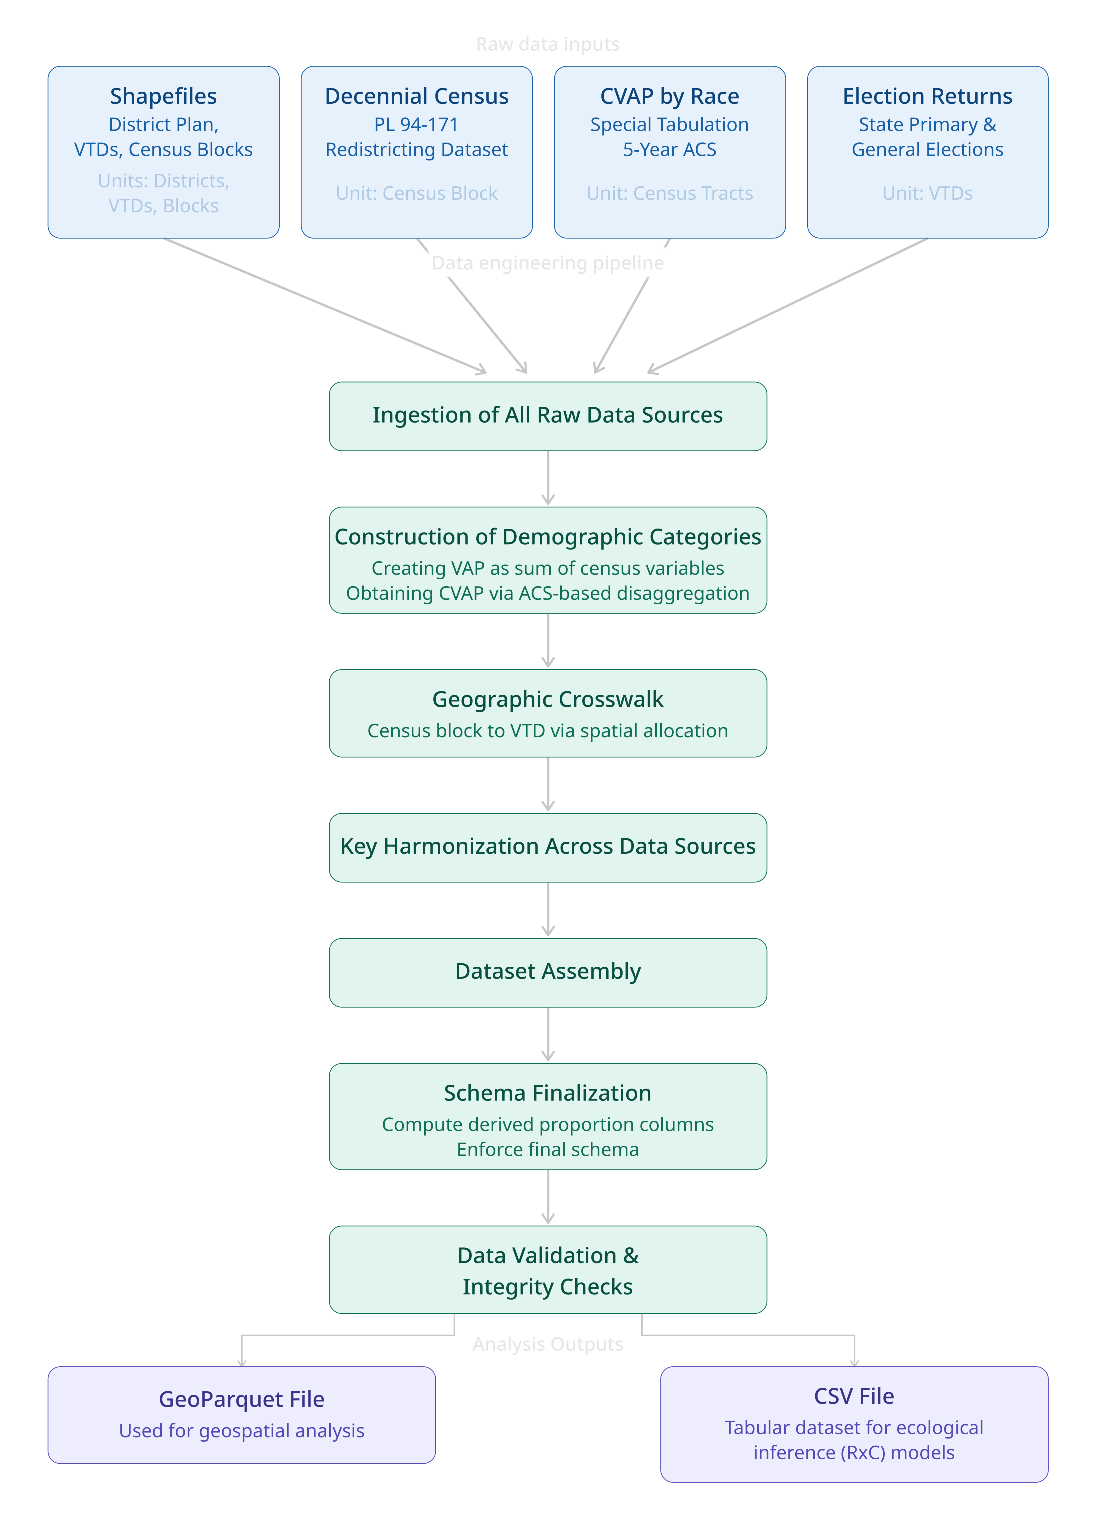
\includegraphics[width=0.9\linewidth]{data_engineering_layer.eps}
    \caption{\textbf{Data Engineering Layer.} An overview of the data engineering layer's end-to-end data engineering pipeline which constructs unified, analysis-ready geospatial and tabular datasets out of ACS, Census, election, and geospatial datasets.}
    \label{fig:data-engineering-layer}
\end{figure}



\subsection{Ecological Inference Layer}
\label{sec:ecological_inference_layer}




\begin{figure}[t]
\centering
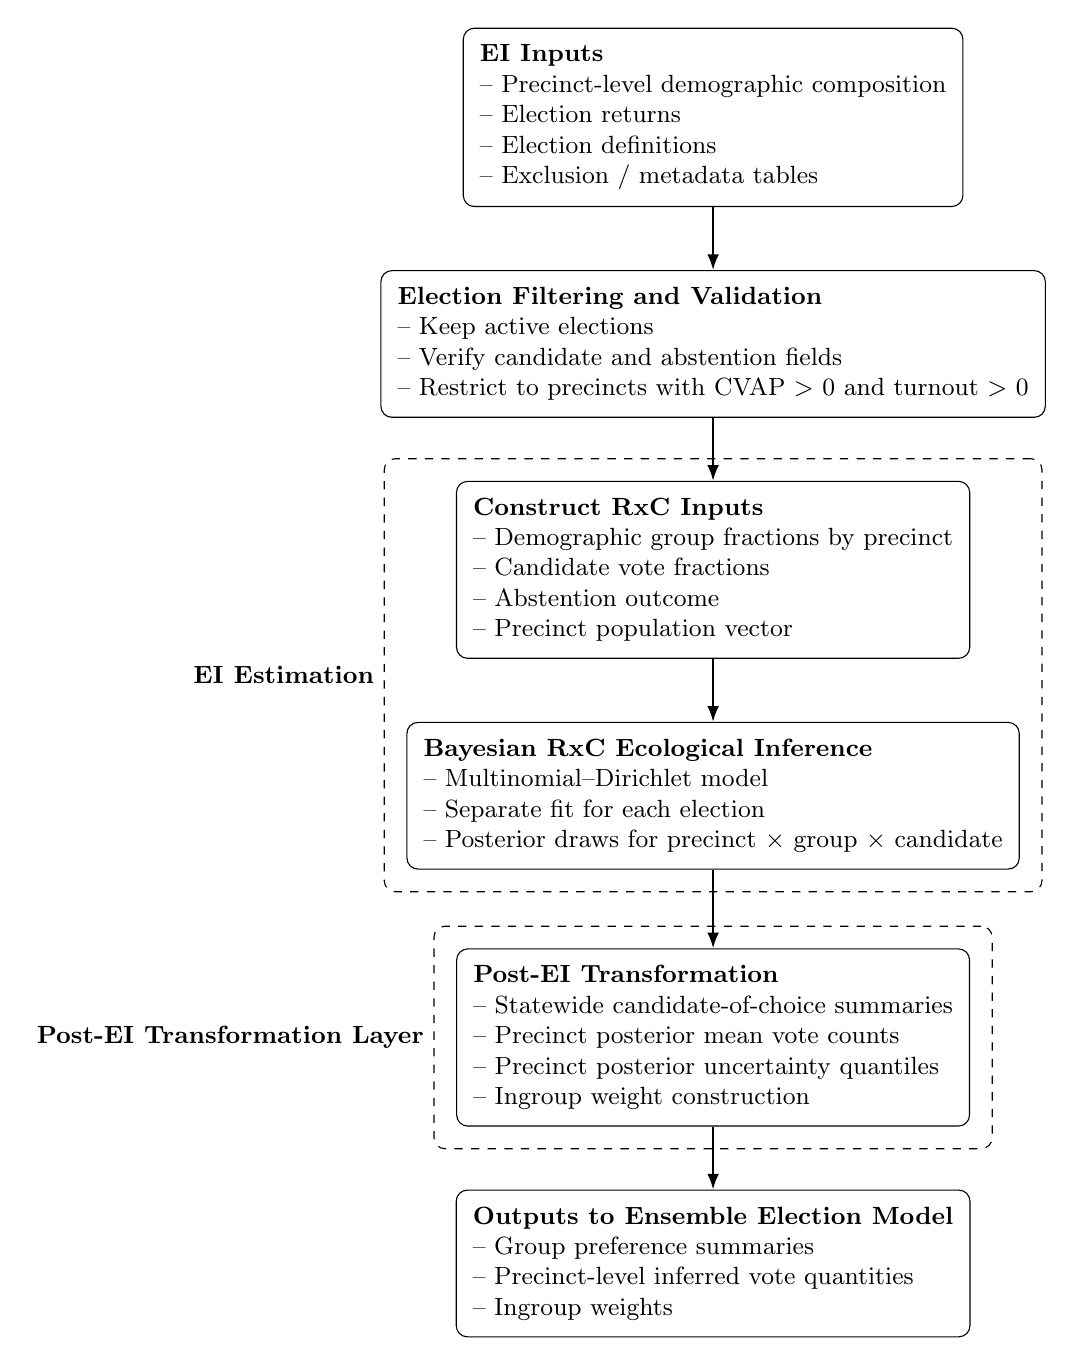
\begin{tikzpicture}[
    node distance=0.8cm and 0.7cm,
    every node/.style={font=\small},
    box/.style={
        draw,
        rounded corners,
        align=left,
        minimum width=5.2cm,
        inner sep=6pt
    },
    stage/.style={
        draw,
        rounded corners,
        dashed,
        inner sep=8pt
    },
    arrow/.style={-{Latex[length=2mm]}, thick}
]

\node[box] (inputs) {
\textbf{EI Inputs}\\
-- Precinct-level demographic composition\\
-- Election returns\\
-- Election definitions\\
-- Exclusion / metadata tables
};

\node[box, below=of inputs] (filter) {
\textbf{Election Filtering and Validation}\\
-- Keep active elections\\
-- Verify candidate and abstention fields\\
-- Restrict to precincts with CVAP $>$ 0 and turnout $>$ 0
};

\node[box, below=of filter] (construct) {
\textbf{Construct RxC Inputs}\\
-- Demographic group fractions by precinct\\
-- Candidate vote fractions\\
-- Abstention outcome\\
-- Precinct population vector
};

\node[box, below=of construct] (model) {
\textbf{Bayesian RxC Ecological Inference}\\
-- Multinomial--Dirichlet model\\
-- Separate fit for each election\\
-- Posterior draws for precinct $\times$ group $\times$ candidate
};

\node[stage, fit=(construct)(model), label=left:{\textbf{EI Estimation}}] {};

\node[box, below=1.0cm of model] (postei) {
\textbf{Post-EI Transformation}\\
-- Statewide candidate-of-choice summaries\\
-- Precinct posterior mean vote counts\\
-- Precinct posterior uncertainty quantiles\\
-- Ingroup weight construction
};

\node[box, below=of postei] (handoff) {
\textbf{Outputs to Ensemble Election Model}\\
-- Group preference summaries\\
-- Precinct-level inferred vote quantities\\
-- Ingroup weights
};

\node[stage, fit=(postei), label=left:{\textbf{Post-EI Transformation Layer}}] {};

\draw[arrow] (inputs) -- (filter);
\draw[arrow] (filter) -- (construct);
\draw[arrow] (construct) -- (model);
\draw[arrow] (model) -- (postei);
\draw[arrow] (postei) -- (handoff);

\end{tikzpicture}
\caption{Ecological inference layer with post-EI transformation. Precinct-level demographic and electoral inputs are converted into row-by-column quantities for a multinomial--Dirichlet Bayesian ecological inference model. Posterior outputs are then transformed into statewide preference summaries, precinct-level inferred vote quantities, uncertainty summaries, and ingroup weights for downstream ensemble analysis.}
\label{fig:ei_postei_layer}
\end{figure}


\subsection{Ensemble Generation Layer}
\subsection{Statistical Comparison Layer}

\section{Mathematical Modeling}
This section formalizes the four computational layers of the framework.

\subsection{Data Engineering Layer}
\subsubsection{Notation and Index Sets}
Let $\mathcal{B}$ denote the set of 2020 Census blocks, indexed by $b$, and let $\mathcal{V}$ denote the set of Voting Tabulation Districts (VTDs), indexed by $v$. Let $\mathcal{T}$ denote the set of Census tracts, indexed by $t(b)$ where $t(b)$ is the tract containing block $b$. All demographic quantities are defined for the Voting-Age Population (VAP) unless noted otherwise.
\subsubsection{Block-Level CVAP Construction}
Following Donnay, Duchin & Rock (n.d.), each racial/ethnic group is defined to be mutually exclusive using a priority ordering: Black → Hispanic → Asian/NHPI → American Indian/Alaska Native (AMIN) → Other → White. Let $\mathcal{C}_g$ denote the set of PL 94-171 Census column codes assigned to group $g$. For each block $b$, the group VAP quantities are:

\begin{equation}
\text{VAP}_b = P3{:}001_b
\label{eq:vap_b}
\end{equation}

\begin{equation}
\text{BVAP}_b = \sum_{c \in \mathcal{C}_B} P3{:}c_b
\label{eq:bvap_b}
\end{equation}


where $\mathcal{C}_B$ contains the 32 PL Table P3 columns that include any Black racial designation (see Donnay et al., Table 1).

For Hispanic VAP, the MGGG convention takes the difference between total VAP (Table P3) and non-Hispanic VAP (Table P4) across 31 multiracial combinations that do not include Black:

\begin{equation}
\text{HVAP}_b = \sum_{(c_3, c_4) \in \mathcal{C}_H} \left( P3{:}c_{3,b} - P4{:}c_{4,b} \right)
\label{eq:hvap_b}
\end{equation}

For the Asian/NHPI (AVAP), AMIN (AMINVAP), and Other (OVAP) groups, the estimator sums the corresponding non-Hispanic P4 columns:

\begin{equation}
\text{XVAP}_b = \sum_{c \in \mathcal{C}_X} P4{:}c_b, \quad X \in \{\text{A, AMIN, O}\}
\label{eq:xvap_b}
\end{equation}


Non-Hispanic single-race White VAP is taken directly from the single P4 column:

\begin{equation}
\text{WVAP}_b = P4{:}005_b
\label{eq:wvap_b}
\end{equation}

Per the MGGG convention, Other VAP is folded with White for the purposes of CVAP estimation (see §3.1.3 below).

\subsubsection{CVAP Estimation via ACS Citizenship Rate "Discounting"}
Because the decennial census does not report citizenship, Citizen Voting-Age Population (CVAP) is estimated at the block level by applying tract-level citizenship rates derived from the ACS 5-year CVAP Special Tabulation. Let $\text{GVAP}^\text{ACS}_{t}$ and $\text{GCVAP}^\text{ACS}_{t}$ denote the ACS group-level VAP and CVAP respectively in tract $t$. The tract-level citizenship rate for group $g$ is:

\begin{equation}
\hat{r}^g_t = \frac{\text{GCVAP}^\text{ACS}_t}{\text{GVAP}^\text{ACS}_t}
\label{eq:tractlevelcitizenshiprate}
\end{equation}

The block-level CVAP for group $g$ is then estimated as:

\begin{equation}
\text{GCVAP}_b = \hat{r}^g_{t(b)} \cdot \text{GVAP}^\text{PL}_b
\label{eq:blocklevelcvap}
\end{equation}

where the "discount" factor $\hat{r}^g_{t(b)}$ is the tract-level citizenship rate matched to the tract $t(b)$ containing block $b$. A state-level fallback rate $\hat{r}^g_{\text{state}}$ is substituted when the tract-level denominator is below the minimum sample threshold $\tau = 20$:

\begin{equation}
\hat{r}^g_{t(b)} = \begin{cases} \dfrac{\text{GCVAP}^\text{ACS}_{t(b)}}{\text{GVAP}^\text{PL}_{t(b)}} & \text{if } \text{GVAP}^\text{PL}_{t(b)} \geq \tau \\[10pt] \hat{r}^g_{\text{state}} & \text{otherwise} \end{cases}
\label{eq:discounting}
\end{equation}

where the state-level rate is $\hat{r}^g_{\text{state}} = \sum_t \text{GCVAP}^\text{ACS}_t \,/\, \sum_b \text{GVAP}^\text{PL}_b$.

Following the MGGG "folded Other" convention, Other VAP shares the White citizenship rate ($\hat{r}^\text{W}$), with the common denominator being $\text{WVAP}_b + \text{OVAP}_b$. Each estimated CVAP is capped at its corresponding VAP to prevent ACS rounding artifacts from producing $\text{GCVAP}_b > \text{GVAP}_b$:

\begin{equation}
\text{GCVAP}_b \leftarrow \min\!\left(\text{GCVAP}_b,\; \text{GVAP}_b\right)
\end{equation}

Total CVAP at the block level is then:

\begin{equation}
\text{CVAP}_b = \sum_{g \in \{B,H,A,\text{AMIN},W\}} \text{GCVAP}_b  
\end{equation}

\subsubsection{Spatial Crosswalk: Areal-Weighted Aggregation to VTDs}
Block-level demographic counts are disaggregated to VTDs via area-weighted areal interpolation. All geometries are reprojected to EPSG:3083 (Texas Centric Albers Equal Area) prior to area computation to ensure accurate planar measurement.

Let $A(b)$ denote the area of block $b$ and let $A(b \cap v)$ denote the area of the intersection of block $b$ with VTD $v$. The area weight assigned to block fragment $b \cap v$ is:

\begin{equation}
w_{bv} = \frac{A(b \cap v)}{A(b)}, \quad w_{bv} \in [0, 1]
\end{equation}

The demographic count for group $g$ in VTD $v$ is obtained by summing the weighted block-level counts over all blocks that intersect $v$:

\begin{equation}
\text{GVAP}_v = \sum_{b:\, A(b \cap v) > 0} w_{bv} \cdot \text{GVAP}_b  
\end{equation}

with analogous expressions for each CVAP group. This formulation assumes uniform population distribution within Census blocks, which is a standard and defensible assumption given that blocks are already very small geographic units.

\subsubsection{Derived Racial Proportions}
For each VTD $v$, the racial composition is summarized by group CVAP proportions:

\begin{equation}
\pi^g_v = \frac{\text{GCVAP}_v}{\text{CVAP}_v}, \quad g \in \{W, B, H, A, \text{AMIN}\}  
\end{equation}


where $\sum_g \pi^g_v = 1$ for all $v$ with $\text{CVAP}_v > 0$ (and $\pi^g_v$ is undefined when $\text{CVAP}_v = 0$). These proportions are denoted `white_prop`, `black_prop`, `hisp_prop`, `asian_prop`, and `amin_prop` in the dataset schema.

\subsubsection{Abstain Column Construction}
For each election $e$ with total votes cast $T^e_v$ and total eligible voters $\text{CVAP}_v$ in precinct $v$, the number of estimated non-voters (abstainers) is:

\begin{equation}
\text{Abstain}^e_v = \max\!\left(\text{CVAP}_v - T^e_v,\; 0\right)  
\end{equation}


The floor at zero prevents negative values in the minority of precincts where observed turnout exceeds the ACS CVAP estimate, which can occur due to ACS sampling error. These abstain counts serve as an additional "candidate" column in the ecological inference model (see §3.2.2).

\subsection{Ecological Inference Layer}
\subsubsection{Problem Setup}
Let $R = 5$ denote the number of racial/ethnic groups ($G_1 = \text{Hispanic},\, G_2 = \text{Black},\, G_3 = \text{White},\, G_4 = \text{Asian},\, G_5 = \text{AMIN}$) and let $C$ denote the number of candidates in a given election (including the Abstain category). 

Across $N$ precincts indexed by $i$, the observed data are:
\begin{itemize}
  \item $\mathbf{x}_i = (\pi^1_i, \ldots, \pi^R_i)^\top$: the vector of group demographic fractions, where $\sum_r \pi^r_i = 1$.
  \item $\mathbf{y}_i = (y^1_i, \ldots, y^C_i)^\top$: the vector of vote-share fractions, where $y^c_i = V^c_i / N_i$, $V^c_i$ is the vote count for candidate $c$ in precinct $i$, and $N_i = \sum_c V^c_i$ is the total votes cast (including abstentions).
  \item $N_i$: the precinct population used as the weight in the model (rounded CVAP).
\end{itemize}


\subsubsection{Multinomial Dirichlet Priors}
The pipeline implements the $R \times C$ Multinomial-Dirichlet ecological inference model of Rosen et al. (2001) as described in Becker, Duchin, Gold & Hirsch (2021), using the Python implementation `pyei.r_by_c.RowByColumnEI` (equivalent to `eiPack::ei.MD.bayes` in R).

Let $\beta^r_i = (\beta^{r,1}_i, \ldots, \beta^{r,C}_i)^\top$ be the (latent, unobserved) vector of voting preferences for group $r$ in precinct $i$, where $\beta^{r,c}_i$ represents the probability that a randomly selected member of group $r$ in precinct $i$ votes for candidate $c$. By definition, $\sum_c \beta^{r,c}_i = 1$ for all $r, i$.

The model is identified through the ecological constraint that the observed precinct-level vote shares are a demographic mixture of the latent group-level preferences:

\begin{equation}
\mathbf{y}_i = \sum_{r=1}^{R} \pi^r_i \, \boldsymbol{\beta}^r_i + \boldsymbol{\varepsilon}_i
\label{eq:aggregation_constraint}
\end{equation}

or equivalently in terms of vote counts:

\begin{equation}
V^c_i \;\Big|\; \{\beta^{r,c}_i\}_{r=1}^{R},\, N_i \;\sim\; \text{Multinomial}\!\left(N_i,\; \sum_{r=1}^{R} \pi^r_i \,\beta^{r,c}_i\right)
\label{eq:vote_counts_constraint}
\end{equation}

Each row $\boldsymbol{\beta}^r_i$ is drawn independently from a group-specific Dirichlet prior:

\begin{equation}
\boldsymbol{\beta}^r_i \;\Big|\; \boldsymbol{\alpha}^r \;\sim\; \text{Dirichlet}\!\left(\boldsymbol{\alpha}^r\right), \qquad r = 1, \ldots, R
\label{eq:hierarchical_prior}
\end{equation}

where $\boldsymbol{\alpha}^r = (\alpha^{r,1}, \ldots, \alpha^{r,C}) \in \mathbb{R}^C_{>0}$ are the concentration parameters of the Dirichlet distribution, shared across precincts within each group. This hierarchical structure allows information to be pooled across precincts while permitting precinct-level heterogeneity in $\boldsymbol{\beta}^r_i$.

The concentration parameters $\boldsymbol{\alpha}^r$ receive weakly informative hyperpriors; the exact form follows the defaults of the `pyei` implementation.

The joint posterior over all latent quantities is:
\begin{equation}
p\!\left(\{\boldsymbol{\beta}^r_i\},\, \{\boldsymbol{\alpha}^r\} \;\Big|\; \{\mathbf{y}_i\},\, \{\mathbf{x}_i\},\, \{N_i\}\right) \propto \prod_{i=1}^{N} \prod_{r=1}^{R} p(\boldsymbol{\beta}^r_i \mid \boldsymbol{\alpha}^r)\; p(\mathbf{y}_i \mid \boldsymbol{\beta}^r_i, \mathbf{x}_i, N_i) \cdot \prod_{r=1}^{R} p(\boldsymbol{\alpha}^r)
\label{eq:posterior_inference}
\end{equation}


This posterior is sampled via MCMC using the No-U-Turn Sampler (NUTS) with $S = 1{,}000$ posterior draws retained per chain after $T = 100{,}000$ tuning steps.

\subsubsection{Posterior Summaries}
Let $\hat{\boldsymbol{\beta}}^{r,c}_{i,s}$ denote the $s$-th posterior draw of group $r$'s support for candidate $c$ in precinct $i$. The estimated statewide support of group $r$ for candidate $c$ is computed as a population-weighted average across precincts:

\begin{equation}
\hat{\mu}^{r,c} = \frac{1}{S} \sum_{s=1}^{S} \frac{\sum_{i=1}^{N} \pi^r_i N_i \,\hat{\beta}^{r,c}_{i,s}}{\sum_{i=1}^{N} \pi^r_i N_i}
\label{eq:statewide_group_preferences}
\end{equation}


where $\pi^r_i N_i$ is the estimated population of group $r$ in precinct $i$.

 For each posterior draw $s$, the candidate of choice for group $r$ is the candidate with the highest weighted support:

\begin{equation}
\text{CoC}^r_s = \arg\max_c \sum_{i=1}^{N} \pi^r_i N_i \,\hat{\beta}^{r,c}_{i,s}
\label{equation:coc}
\end{equation}


The fraction of draws in which each candidate is the candidate of choice, $\hat{p}^{r,c} = S^{-1}\sum_s \mathbf{1}[\text{CoC}^r_s = c]$, is reported alongside the mean support $\hat{\mu}^{r,c}$ as a measure of posterior certainty.

The expected number of votes cast by group $r$ for candidate $c$ in precinct $i$ is estimated as:

\begin{equation}
\hat{m}^{r,c}_i = \frac{1}{S} \sum_{s=1}^{S} \hat{\beta}^{r,c}_{i,s} \cdot \pi^r_i N_i
\label{eq:precinctlevelmeanvotecounts}
\end{equation}

The posterior distribution of vote counts for group $r$, candidate $c$, precinct $i$ across draws $s$ is summarized by octile quantiles at probabilities $\{k/8 : k = 1, \ldots, 8\}$:

\begin{equation}
\hat{Q}^{r,c}_{i,k} = \text{Quantile}_{k/8}\!\left(\hat{\beta}^{r,c}_{i,s} \cdot \pi^r_i N_i\right)_{s=1}^{S}
\label{eq:precinctlevelquantiles}
\end{equation}

These quantile estimates enable uncertainty quantification at the precinct level and are used in downstream VRA Section 2 analyses.

\subsubsection{Summary of Model Inputs and Outputs}
| Symbol | Quantity | Source |
|---|---|---|
| $\text{GVAP}_b$ | Group voting-age population, block $b$ | PL 94-171 |
| $\hat{r}^g_t$ | Group citizenship rate, tract $t$ | ACS CVAP Special Tabulation |
| $\text{GCVAP}_b$ | Estimated group CVAP, block $b$ | Discounting (§3.1.3) |
| $w_{bv}$ | Area weight, block $b$ to VTD $v$ | TIGER/LINE geometry (§3.1.4) |
| $\pi^g_v$ | Group CVAP fraction, VTD $v$ | §3.1.5 |
| $\text{Abstain}^e_v$ | Non-voter count, election $e$, VTD $v$ | §3.1.6 |
| $\boldsymbol{\beta}^r_i$ | Latent group voting preferences | EI posterior (§3.2.2) |
| $\hat{\mu}^{r,c}$ | Statewide group support for candidate $c$ | §3.2.3 |
| $\hat{Q}^{r,c}_{i,k}$ | Precinct-level posterior octiles | §3.2.3 |


\section{Case Study: Texas Congressional Districts}
\subsection{Data Engineering Layer Implementation}

\begin{table}[ht]
\centering
\caption{Texas Demographics}
\begin{tabular}{lccc}
\hline
\textbf{Racial Group} & \textbf{Share of Total Population} & \textbf{Share of VAP} & \textbf{Share of CVAP} \\
\hline
Hispanic & 34.7\% & 35.6\% & 32.6\% \\
Black  & 13.5\% & 13.0\% & 12.9\% \\
White  & 46.2\% & 43.2\% & 48.9\% \\
Asian  & 5.0\%  & 6.1\%  & 4.8\% \\
American Indian  & 0.7\%  & 1.3\%  & 0.7\% \\
\hline
\textit{Total Count} &  29,145,505 &  21,866,700 &  18,252,793\\
\hline
\end{tabular}

\vspace{0.5em}
\footnotesize{
Latino, Black, White, and Other shares of Texas residents by total population, voting-age population (VAP), and citizen voting-age population (CVAP). 
Total population and VAP data are taken from the 2020 decennial census, while CVAP data come from the American Community Survey (ACS) five-year rolling average ending in 2024.
}
\end{table}

\begin{table}[ht]
\centering
\caption{The 3 Election Sets in the Texas Data}
\begin{tabular}{lcccc}
\toprule
Office & Stage & Year \\
\midrule
President & General & 2024 \\
President & Primary & 2024 \\
U.S. Senate & General & 2024 \\ 
U.S. Senate & Primary & 2024 \\
Railroad Commissioner & General & 2024 \\ 
Railroad Commissioner & Primary & 2024 \\

\bottomrule
\end{tabular}

\vspace{0.5em}
\begin{minipage}{0.9\textwidth}
\footnotesize
The 3 election sets in our Texas data.
\end{minipage}

\end{table}

\subsection{Ecological Inference Layer Implementation}
\subsubsection{Ensemble Generation Layer Implementation}
\subsubsection{Statistical Comparison Layer}


\section{Discussion}\label{sec12}


\section{Conclusion}\label{sec13}


\backmatter




\bmhead{Acknowledgements}
I am indebted to the SoReMo Initiative at my home institution, Illinois Institute of Technology, for funding my research. Dr. Sonja Petrović, founder of the SoReMo Initiative, has provided invaluable statistical insights. Dr. Robert Ellis, my advisor, has provided candid and thorough throughout the formulation of this paper. Dr. Shahrzad (Sara) Jamshidi, my statistics professor, was instrumental in helping me get this project off the ground. 

\section*{Declarations}
Not applicable.


\bigskip



%%===========================================================================================%%
%% If you are submitting to one of the Nature Portfolio journals, using the eJP submission   %%
%% system, please include the references within the manuscript file itself. You may do this  %%
%% by copying the reference list from your .bbl file, paste it into the main manuscript .tex %%
%% file, and delete the associated \verb+\bibliography+ commands.                            %%
%%===========================================================================================%%

\bibliography{sn-bibliography}% common bib file
%% if required, the content of .bbl file can be included here once bbl is generated
%%\input sn-article.bbl


\end{document}
